\documentclass{article}
\usepackage{graphicx}
\usepackage{amsmath}
\usepackage{amsfonts}
\usepackage{bookmark}
\usepackage{booktabs}
\usepackage{exercises}
\graphicspath{ {} }
\usepackage{indentfirst}
\usepackage{amsthm}
\usepackage{yhmath}
\usepackage{geometry}
\usepackage{placeins}
\usepackage{csquotes}
\usepackage{pgfplots}
\newcommand*{\oldneg}{\mathord{\sim}}
\newcommand\showdiv[1]{\overline{\smash{)}#1}}
\newcommand\Mydiv[1]{%
\smash{\raise.3ex\hbox{$\big)$}}\mkern-8mu
        \overline{\enspace\strut#1}}
\setlength{\tabcolsep}{5pt}
\theoremstyle{definition}
\newtheorem{definition}{Definition}

\setlength{\parindent}{.5in}
\setlength{\parskip}{12pt}
\renewcommand{\arraystretch}{2}
\geometry{margin=1in}
\newcommand{\?}{\stackrel{?}{=}}
\pgfplotsset{width=7cm,compat=1.18}\usepgfplotslibrary{statistics}

\title{6.2 Answers}
\begin{document}
\maketitle

\section*{Problem 1}
A probability distribution represented by a histogram is symmetric if you can draw a vertical line dividing the histogram into two parts that 
are mirror images.

\section*{Problem 2}
A binomial experiment is some experiment satisfying the following conditions:\newline
(1): There are $n$ independent trials.\newline
(2): Every trial can have only two possible outcomes: success or failure.\newline
(3): The probability for succes, denoted by $p$, is the same for each trial. The probability of failure is given by $1-p$.\newline
A binomial distribution shows the probabilities of the outcomes of a given binomial experiment.

\section*{Problem 5}
\begin{center}
\begin{tabular}{l|l|l}
Digits & Occurences & $P(X)$ \\
$1$ & $10$ & $\frac{10}{1000}=\frac{1}{100}$ \\
\cmidrule{1-3}
$2$ & $90$ & $\frac{90}{1000}=\frac{9}{100}$ \\
\cmidrule{1-3}
$3$ & $900$ & $\frac{900}{1000}=\frac{9}{10}$ \\
\end{tabular}
\end{center}

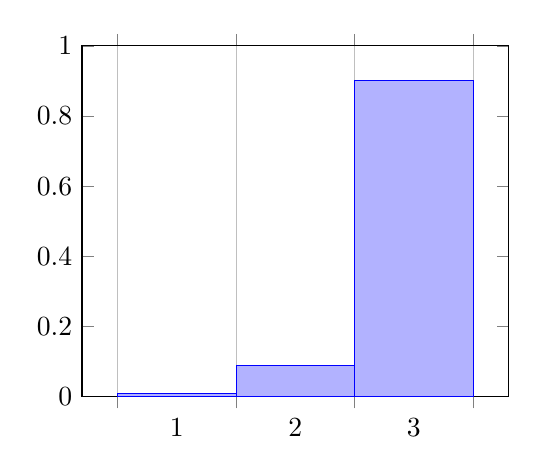
\begin{tikzpicture}
\begin{axis}[ybar interval, ymax=1,ymin=0]
\addplot+ plot coordinates { (1, 1/100) (2, 9/100) (3, 9/10) (4, 0) };
\end{axis}
\end{tikzpicture}

\section*{Problem 16}
We can create a binomial experiment for tossing a coin, and getting heads. The chance of getting heads is 50 percent, and thus, if we are tossing it 
20 times, the probability of getting 15 heads is: 
\[ _{20}C_{15}\times 0.5^{15}\left(1-0.5\right)^{20-15}=15504\times 0.5^{15}(0.5)^{5}\approx 0.015 \] meaning the probability is about $1.5$ percent.

\section*{Problem 17}
We can use the same binomial experiment as in Problem 16, and conclude that the probability for $18$ heads is
\[ _{20}C_{18}\times 0.5^{18}\left(1-0.5\right)^{20-18}=190\times 0.5^{18}\times 0.5^{2}\approx 0.00018 \] meaning the probability is about 
$0.018$ percent.

\section*{Problem 23}
We can set up a binomial experiment for the given situation, in which the change of guessing right is 25 percent, and such that there are 30 tests.
\[ _{30}C_{21}\times 0.25^{21}\times 0.75^{30-21}=14307150\times 0.25^{21}\times 0.75^{9}\approx 0.00000024 \] meaning the probability is about 
$0.000024$ percent for guessing 21 correctly.

\section*{Problem 25}
This can be done using the same binomial experiment as in Problem 25:
\[ _{30}C_{30}\times 0.25^{30}\times 0.75^{30-30}=0.25^{30}\approx 0.00000000000000000087 \] meaning the probability is about
$0.000000000000000087$ percent.

\section*{Problem 30}
We are searching for the probabiltiy of $k$ successes, that is, when $k\le 2$, so we can check the probabilities for $0,1$ and $2$.\newline
$k=0$: $_5C_0\times 0.12^0\times (1-0.12)^5\approx 0.53$\newline
$k=1$: $_5C_1\times 0.12^1\times (1-0.12)^4\approx 0.36$\newline
$k=2$: $_5C_2\times 0.12^2\times (1-0.12)^3\approx 0.10$\newline
Meaning the probability when $k\le 2$ is $0.53+0.36+0.10=.99$ or about $99$ percent.

\section*{Problem 33}
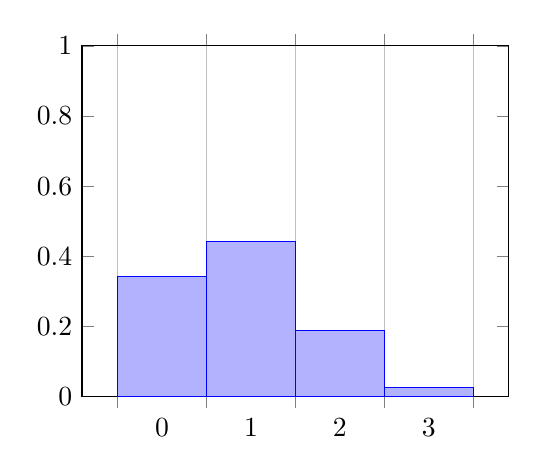
\begin{tikzpicture}
\begin{axis}[ybar interval, ymax=1,ymin=0]
\addplot+ plot coordinates { (0, 0.343) (1, 0.441) (2, 0.189) (3, 0.027) (4,0) };
\end{axis}
\end{tikzpicture}
\newline
From the histogram, we can see that the distribution is skewed. The most likely number of successes is $1$.

\section*{Problems 40-42}
We consider some particular sequence of $k$ successess and $n-k$ failure. For each given member in the sequence, there is a $(1-p)$ chance of failure, and a $p$ chance of 
success. Hence there would be a probability of $(1-p)^{n-k}$ for the given number of failures to occur, and a probability of $p^k$ for the given number of successes to occur, meaning the 
sequence itself has a probability of $p^k(1-p)^{n-k}$ to occur.


If we consider $n$ objects and $k$ successes, there are $_nC_k$ ways in which to choose the successes (and thus the entire sequence), as the order of the successes themselves does not matter.
The binomial probability formula shows the probability for one of the sequences of $k$ successes and $n-k$ failures to occur. Because there are $_nC_k$ ways in which to choose such a 
sequence, and each one of those sequences has a $p^k(1-p)^{n-k}$ probability of occuring, the probability of any one of those sequences to occur is
$_nC_kp^k(1-p)^{n-k}$.


\section*{Problem 48}
(a): We are given that the probability of having a boy or girl is equal, meaning the statement \textquote{The first 4 kids were all boys, so the next one will probably be a girl."} is not 
correct, as it is equally probable that it would be a girl or a boy.


(b): We are given that the probability of having a boy or girl is equal (0.5). Set up a binomial experiment in the following way: a success is having a 
girl, while a failure is having a boy. Hence, we need to determine the chance of having $5$ failures (that is, 5 boys in a row):
\[ _5C_0\times 0.5^0\times 0.5^5\approx 0.03125 \] meaning the probability of not having $5$ failures (meaning having the fifth child be a girl) is:
$1-0.03125=0.96875$, or about $96.9$ percent. Hence, the given event is probable.


(c): The probabilities for having a female child after having each of the given numbers of male children already had can be found in a similar way to 
the first two sections, except now we are interested in the probability of having a $male$ for the first $k$ times, not a female:\newline
$0$: $0.5$\newline
$1$: $0.5^2=0.25$\newline
$2$: $0.5^3=0.125$\newline
$3$: $0.5^4=0.0625$\newline
$4$: $0.5^5=0.03125$\newline
$5$: $0.5^6\approx 0.0157$\newline
$6$: $0.5^7\approx 0.0078$\newline
$7$: $0.5^8\approx 0.0039$\newline
$8$: $0.5^9\approx 0.00195$\newline
$9$: $0.5^{10}\approx 0.00098$\newline
$10$: $0.5^{11}\approx 0.00049$\newline
thus meaning a histogram to represent the situation is:\newline
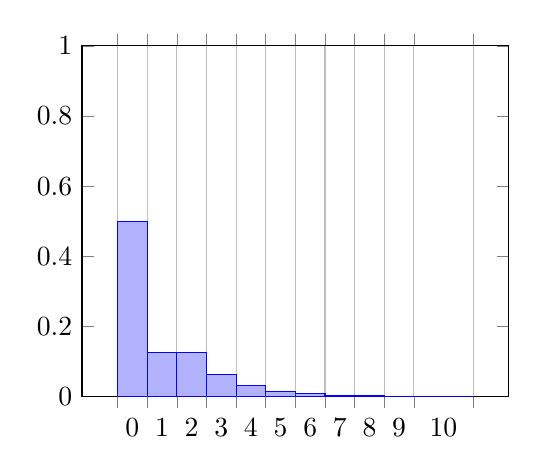
\begin{tikzpicture}
\begin{axis}[ybar interval, ymax=1,ymin=0]
\addplot+ plot coordinates { (0, 0.5) (1, 0.125) (2, 0.125) (3,0.0625) (4,0.03125) (5,0.0157) (6,0.0078) (7,.0039) (8,.00195) (9,.00098) (10,.00049) (12,0) };
\end{axis}
\end{tikzpicture}
\newline
This is a skewed histogram.

\section*{Problem 49}
(I produced an inequality which I think is correct, but I could not solve it)\newline
We are comparing a 3-speaker to a 5-speaker system. We are given that the system will work properly if at least 50\% of it's speakers are functioning properly. Each speaker will function 
with probability $p$, independent of whether the other speakers are functioning. Thus we can create a binomial experiment for the two systems. For the first system
(one with 3 speakers), the probability that the system will function properly is: \[ _3C_2p^2(1-p)+p^3 \] while the probability that the system with 5 speakers will function properly is:
\[ _5C_3p^3(1-p)^2+_5C_4p^4(1-p)+p^5 \] We are trying to figure out what values of $p$ make the 5-speaker system more likely to operate than the 3-speaker system. Thus we need to solve the 
inequality:
\[ _5C_3p^3(1-p)^2+_5C_4p^4(1-p)+p^5>_3C_2p^2(1-p)+p^3 \]
\[ 10p^3(1-p)^2+5p^4(1-p)+p^2>3p^2(1-p) \]
\[ 10p^6-20p^4+10p^3+5p^4-5p^5+p^2>3p^2-3p^3 \]
\[ 10p^6-5p^5-15p^4+13p^3-2p^2>0 \]

\end{document}
